\documentclass[a4paper, 12pt]{article}
\usepackage[utf8]{inputenc}
\usepackage[spanish]{babel}
\usepackage{amsmath}
\usepackage{amsfonts}
\usepackage{amssymb}
\usepackage{geometry}
\usepackage{listings}
\usepackage{xcolor}
\usepackage{hyperref}
\usepackage{fancyvrb}
\usepackage{graphicx}

\geometry{
 a4paper,
 total={170mm,257mm},
 left=20mm,
 top=20mm,
}

\definecolor{codegray}{rgb}{0.5,0.5,0.5}
\definecolor{codepurple}{rgb}{0.58,0,0.82}
\definecolor{backcolour}{rgb}{0.98,0.98,0.98}
\definecolor{keywordcolor}{rgb}{0.13,0.13,1.0}

\lstdefinestyle{pythonstyle}{
  backgroundcolor=\color{backcolour},
  commentstyle=\color{codegray},
  keywordstyle=\color{keywordcolor},
  numberstyle=\tiny\color{codegray},
  stringstyle=\color{codepurple},
  basicstyle=\footnotesize\ttfamily,
  breakatwhitespace=false,
  breaklines=true,
  captionpos=b,
  keepspaces=true,
  numbers=left,
  numbersep=5pt,
  showspaces=false,
  showstringspaces=false,
  showtabs=false,
  tabsize=2,
  language=Python,
}
\lstset{style=pythonstyle}

\begin{document}

\begin{titlepage}
    \centering
    \vspace*{2cm} 
    
    
\includegraphics[width=0.8\textwidth]{images/logo_uct.jpg} 

    \vspace{2cm}
    {\Huge \textbf{Informe de Análisis de Código}}
    
    \vspace{0.5cm}
    {\huge Sistema de Gestión de Restaurante}
    
    \vfill
    
    {\Large \textbf{Integrantes:} Nicolás Cayuman, Gabriel Gutiérrez, Ailyn Melillán}
    
    \vspace{0.5cm}
    {\Large \textbf{Asignatura:} Programación II}
    
    \vspace{0.5cm}
    {\Large \textbf{Profesor:} Guido Mellado}
    
    \vspace{0.5cm}
    {\Large \textbf{Ayudante:} Joaquín Cantero}

    \vspace{0.5cm}
    {\Large Ingeniería CIvil en Informática}
    
    \vspace{0.5cm}
    {\Large 15 de Octubre de 2025} 
    
    \vspace{1cm}
\end{titlepage}
\thispagestyle{empty} 
\newpage

\tableofcontents

\newpage

\section{Introducción y Problemática}

El sector de la \textbf{restauración} moderna se enfrenta al desafío constante de optimizar la eficiencia operativa, mejorar la experiencia del cliente y mantener un control riguroso sobre los recursos. La gestión manual de inventario, la toma de pedidos y la emisión de comprobantes son tareas propensas a errores, lentas y que consumen valiosos recursos humanos.

\textbf{Problemática:} Se solicita el desarrollo de una \textbf{interfaz gráfica de usuario (GUI)} moderna y eficiente para un restaurante, con el objetivo de \textbf{digitalizar y centralizar} la gestión de los procesos clave de venta e inventario. Esta aplicación debe:
\begin{itemize}
    \item Mantener un control en tiempo real del \textbf{inventario de ingredientes (Stock)}, soportando la \textbf{carga masiva de datos} desde archivos CSV para una inicialización rápida.
    \item Facilitar la \textbf{toma de pedidos} de manera ágil a partir de un \textbf{catálogo de menús} predefinido.
    \item Asegurar que cada venta \textbf{descuente automáticamente} los ingredientes correspondientes del stock disponible para prevenir ventas sin capacidad de suministro.
    \item Generar automáticamente la \textbf{boleta de venta} y la \textbf{carta del restaurante} en formato digital (PDF) para una documentación clara y profesional.
\end{itemize}
La solución debe ser implementada utilizando \textbf{Python} y la librería \textbf{customtkinter} para ofrecer una estética moderna y una experiencia de usuario robusta.

\newpage

\section{Análisis y Explicación de Archivos \texttt{.py}}

A continuación, se detalla la función y estructura de cada archivo Python que compone el sistema:

\subsection{\texttt{Ingrediente.py}}
\begin{itemize}
    \item \textbf{Propósito:} Define la estructura de datos para un \textbf{ingrediente} individual.
    \item \textbf{Clase Principal:} \texttt{Ingrediente} ($\texttt{@dataclass}$).\\
    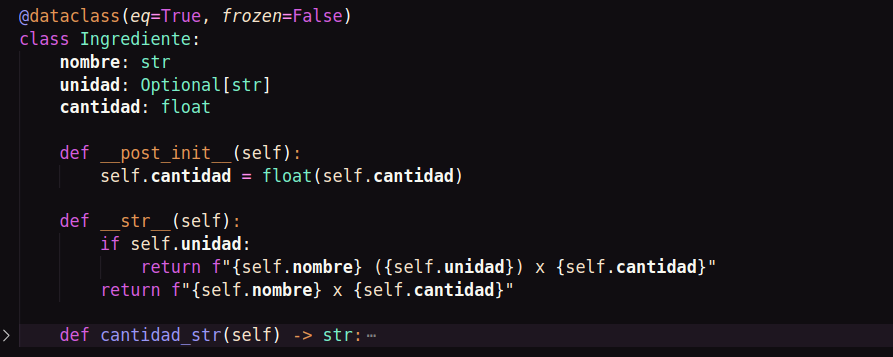
\includegraphics[width=0.8\textwidth]{images/13.png}\\  
    \item \textbf{Funcionalidad Clave:} El método \texttt{cantidad\_str()} formatea la cantidad (float) para su visualización, eliminando el \texttt{.0} innecesario (ej: $5.0 \to '5'$; $5.5 \to '5.5'$), mejorando la presentación en la GUI.*\\

    \begin{lstlisting}[language=Python, caption=Función de cantidad]
def cantidad_str(self) -> str:
        """Devuelve la cantidad como string sin el '.0' innecesario.

        Ejemplos:
        5.0 -> '5'
        5.5 -> '5.5'
        """
        try:
            val = float(self.cantidad)
            if val.is_integer():
                return str(int(val))

            rounded = round(val, 3)
            s = f"{rounded:.3f}".rstrip('0').rstrip('.')
            return s
        
        except Exception:
            return str(self.cantidad)
\end{lstlisting}

\end{itemize}
\newpage
\subsection{\texttt{IMenu.py}}
\begin{itemize}
    \item \textbf{Propósito:} Define un \textbf{Protocolo} (interfaz) que deben seguir los elementos vendibles del menú.
    \item \textbf{Clase Principal:} \texttt{IMenu} ($\texttt{typing.Protocol}$).\\
    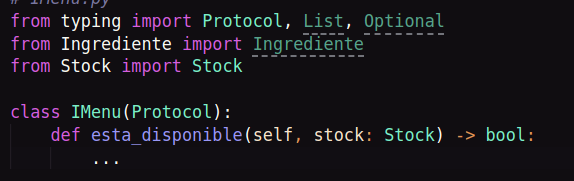
\includegraphics[width=0.8\textwidth]{images/3.png}
    
    \item \textbf{Funcionalidad Clave:} Aunque vacía, su existencia impone una estructura de diseño orientada a la inyección de dependencias, asegurando que las clases de menú cumplan con los requisitos mínimos del sistema.

\end{itemize}
\subsection{\texttt{ElementoMenu.py}}
\begin{itemize}
    \item \textbf{Propósito:} Implementa la clase concreta que representa un elemento del menú que requiere ingredientes.
    \item \textbf{Clase Principal:} \texttt{CrearMenu} ($\texttt{@dataclass}$).  \\
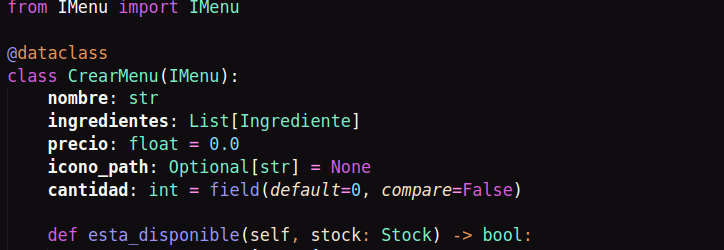
\includegraphics[width=0.8\textwidth]{images/4.png}
    \item \textbf{Funcionalidad Clave:} El método \texttt{esta\_disponible(stock: Stock)} es crucial. Comprueba, iterando sobre los ingredientes requeridos y el \texttt{Stock} disponible, si la cantidad de cada ingrediente es suficiente para preparar el menú.
\end{itemize}
\begin{lstlisting}[language=Python, caption=Función de esta disponible]
    def esta_disponible(self, stock: Stock) -> bool:
        for req in self.ingredientes:
            ok = False
            for ing in stock.lista_ingredientes:
                if ing.nombre == req.nombre and (req.unidad is None or ing.unidad == req.unidad):
                    if int(ing.cantidad) >= int(req.cantidad):
                        ok = True
                        break
            if not ok:
                return False
        return True
\end{lstlisting}

\newpage
\subsection{\texttt{Stock.py}}
\begin{itemize}
    \item \textbf{Propósito:} Gestiona la colección de \texttt{Ingrediente}s y la \textbf{persistencia de datos} mediante un archivo CSV (\texttt{ingredientes\_menu.csv}).
    \item \textbf{Clase Principal:} \texttt{Stock}.\\
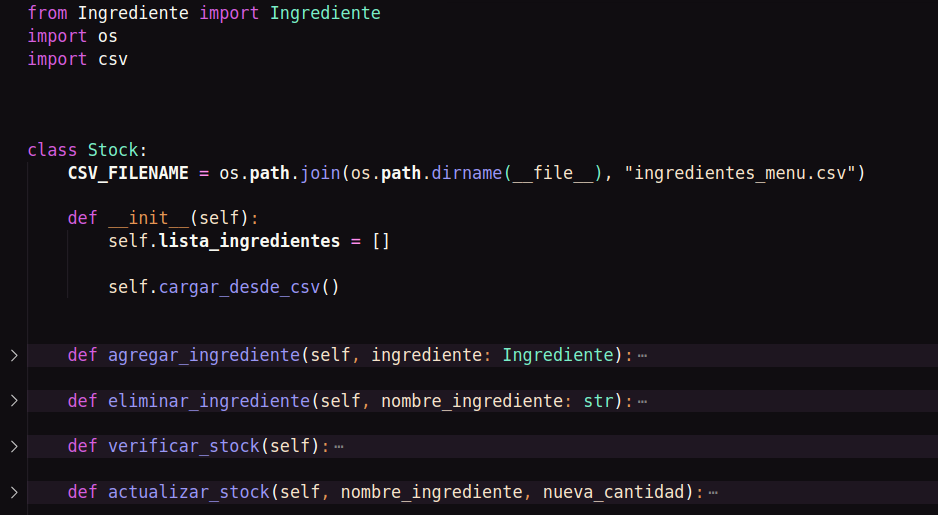
\includegraphics[width=0.8\textwidth]{images/5.png}
    \item \textbf{Funcionalidad Clave:}
    \begin{itemize}
    
        \begin{lstlisting}
            def agregar_ingrediente(self, ingrediente: Ingrediente):
        nombre_nuevo = ingrediente.nombre.strip().lower()
        for ing in self.lista_ingredientes:
            if str(ing.nombre).strip().lower() == nombre_nuevo:
                try:
                    ing.cantidad = float(ing.cantidad) + float(ingrediente.cantidad)
                except Exception:
                
                    try:
                        ing.cantidad = float(ingrediente.cantidad)
                    except Exception:
                        pass
                self.actualizar_csv()
                return True

        try:
            ingrediente.nombre = ingrediente.nombre.strip().capitalize()
        except Exception:
            pass
        self.lista_ingredientes.append(ingrediente)
        self.actualizar_csv()
        return True
        \end{lstlisting}
        
        \item \texttt{agregar\_ingrediente}: Si el ingrediente existe, suma la cantidad; si no, lo añade. 

\newpage

        \begin{lstlisting}
            def cargar_desde_csv(self):
        self.lista_ingredientes = []
        if not os.path.exists(self.CSV_FILENAME):
            return
        
        try:
            with open(self.CSV_FILENAME, newline='', encoding='utf-8') as csvfile:
                reader = csv.DictReader(csvfile)
                for row in reader:
                    nombre = row.get('nombre') or row.get('Name') or row.get('Nombre') or row.get('nombre_ingrediente')
                    unidad = row.get('unidad') or row.get('Unidad') or ''
                    cantidad = row.get('cantidad') or row.get('Cantidad') or 0
                    if nombre:
                        try:
                            ing = Ingrediente(nombre=str(nombre), unidad=str(unidad) if unidad else None, cantidad=float(cantidad))
                        except Exception:
                            
                            try:
                                ing = Ingrediente(nombre=str(nombre), unidad=str(unidad) if unidad else None, cantidad=float(cantidad))
                            except Exception:
                                ing = Ingrediente(nombre=str(nombre), unidad=str(unidad) if unidad else None, cantidad=0)
                        self.lista_ingredientes.append(ing)
        except Exception:   
            pass
        \end{lstlisting}
        
        \item \texttt{cargar\_desde\_csv}: Inicializa el stock leyendo el archivo de persistencia.
    
        \item \texttt{actualizar\_csv}: Persiste el estado actual de la lista de ingredientes en el archivo CSV.
    \end{itemize}
\end{itemize}

\subsection{\texttt{Menu\_catalog.py}}
\begin{itemize}
    \item \textbf{Propósito:} Proporciona la \textbf{carta predefinida} del restaurante.
    \item \textbf{Función Principal:} \texttt{get\_default\_menus()}.\\
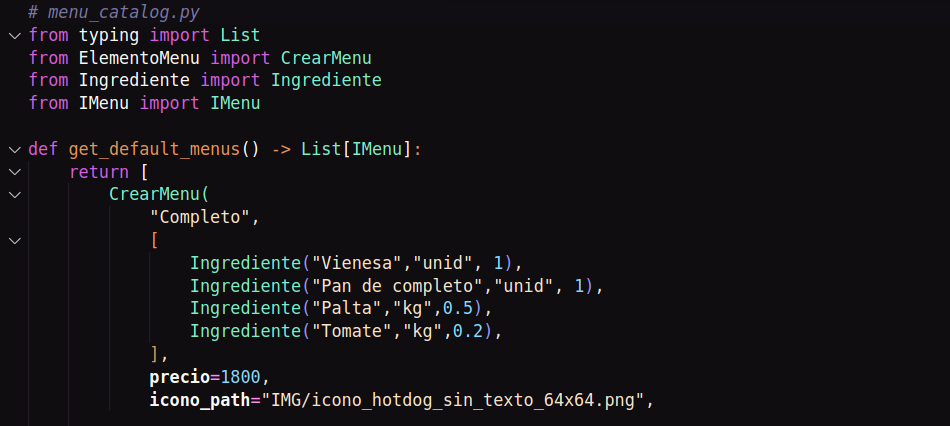
\includegraphics[width=0.8\textwidth]{images/6.png}
    \item \textbf{Funcionalidad Clave:} Retorna una lista de objetos \texttt{CrearMenu} (ej: "Completo", "Chorrillana"), definiendo sus ingredientes requeridos, precio y la ruta de su ícono.
\end{itemize}

\subsection{\texttt{Pedido.py}}
\begin{itemize}
    \item \textbf{Propósito:} Representa el estado actual de la \textbf{orden de un cliente}.
    \item \textbf{Clase Principal:} \texttt{Pedido}.\\
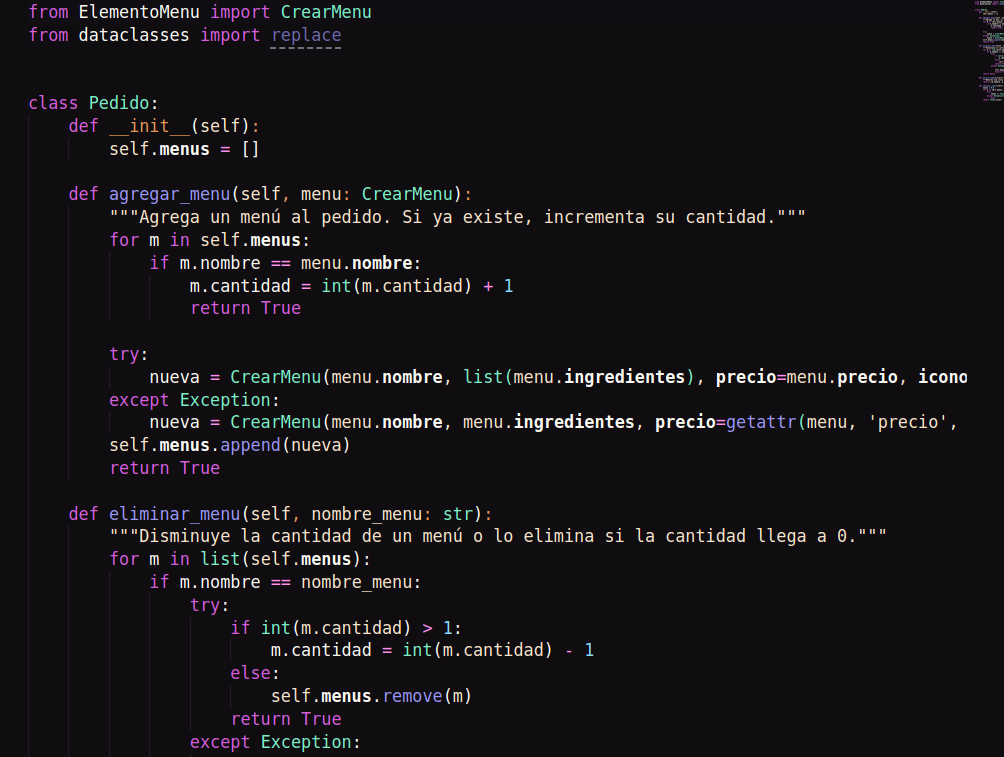
\includegraphics[width=0.8\textwidth]{images/7.png}
    \item \textbf{Funcionalidad Clave:}
    \begin{itemize}
        \item \texttt{agregar\_menu}: Añade o incrementa la cantidad de un menú en el pedido.
        \item \texttt{eliminar\_menu}: Decrementa la cantidad o elimina el menú si la cantidad es 1.
        \item \texttt{calcular\_total}: Calcula el costo total del pedido.
    \end{itemize}
\end{itemize}
\newpage
\subsection{\texttt{BoletaFacade.py}}
\begin{itemize}
    \item \textbf{Propósito:} Facilita la generación de la \textbf{boleta de venta en formato PDF}. Actúa como un patrón \textbf{Fachada} sobre la librería \texttt{fpdf}.
    \item \textbf{Clase Principal:} \texttt{BoletaFacade}.\\
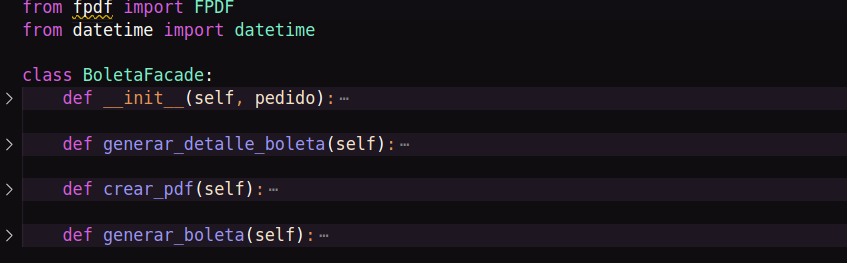
\includegraphics[width=0.8\textwidth]{images/8.png}
    \item \textbf{Funcionalidad Clave:} Coordina los métodos \texttt{generar\_detalle\_boleta} 

    \begin{lstlisting}
         def generar_detalle_boleta(self):
        self.detalle = ""
        for item in self.pedido.menus:
            subtotal = item.precio * item.cantidad
            self.detalle += f"{item.nombre:<30} {item.cantidad:<10} ${item.precio:<10.2f} ${subtotal:<10.2f}\n"
        
        self.subtotal = self.pedido.calcular_total()
        self.iva = self.subtotal * 0.19
        self.total = self.subtotal + self.iva

        def generar_boleta(self):
            """Coordina la generación de la boleta y la creación del PDF."""
            self.generar_detalle_boleta()
            pdf_path = self.crear_pdf()
            return(f"Boleta generada y guardada en: {pdf_path}")

    \end{lstlisting}
    
    (cálculo de subtotal, IVA del 19\% y total) y \texttt{crear\_pdf}, que formatea la información del pedido en el archivo \texttt{boleta.pdf}.
\end{itemize}

\subsection{\texttt{menu\_pdf.py}}
\begin{itemize}
    \item \textbf{Propósito:} Genera un \textbf{PDF con la carta} del restaurante con un diseño estilizado.
    \item \textbf{Función Principal:} \texttt{create\_menu\_pdf}.\\
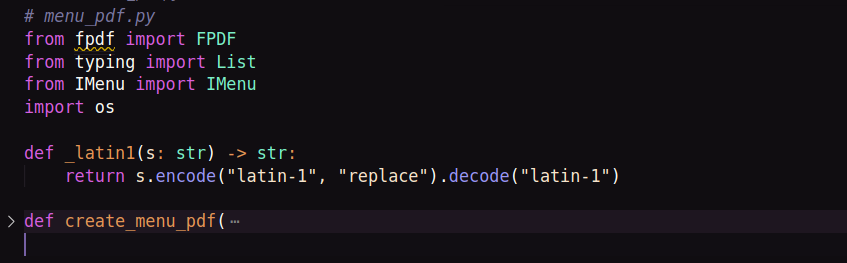
\includegraphics[width=0.8\textwidth]{images/9.png}
    \item \textbf{Funcionalidad Clave:} Utiliza \texttt{fpdf} para crear el archivo \texttt{carta.pdf}. Aplica un diseño profesional con banner, filas alternadas (\textit{zebra}) y precios alineados.
\end{itemize}
\newpage
\subsection{\texttt{ctk\_pdf\_viewer.py}}
\begin{itemize}
    \item \textbf{Propósito:} Proporciona un \textbf{widget} para \textbf{visualizar archivos PDF} dentro de la aplicación \texttt{customtkinter}.\\
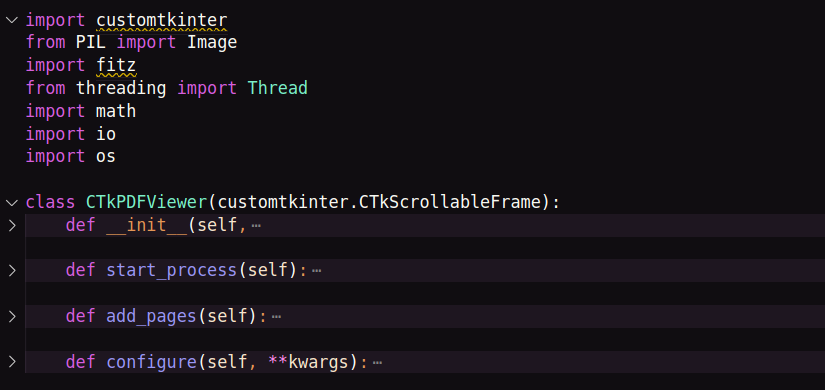
\includegraphics[width=0.8\textwidth]{images/10.png}
    \item \textbf{Clase Principal:} \texttt{CTkPDFViewer} (\textit{Hereda de} \texttt{CTkScrollableFrame}).\\
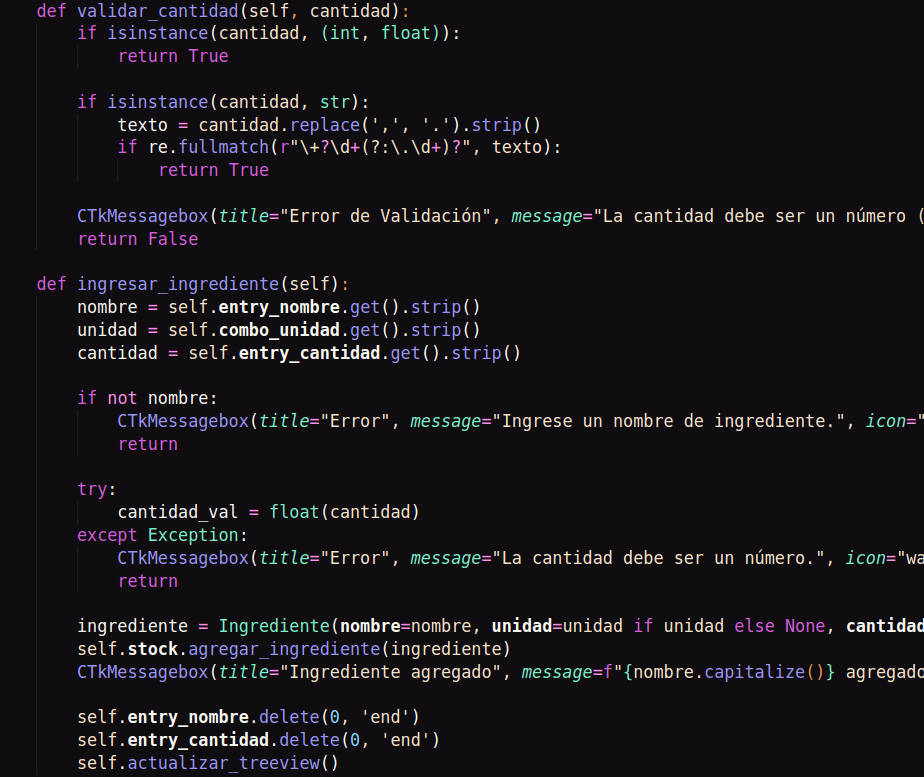
\includegraphics[width=0.8\textwidth]{images/11.png}
    \item \textbf{Funcionalidad Clave:} Utiliza las librerías \texttt{fitz} (PyMuPDF) para renderizar cada página del PDF como una imagen (\texttt{CTkImage}). La carga se realiza en un \textbf{hilo separado} (\texttt{threading}) para no congelar la GUI, mostrando una barra de progreso.
\end{itemize}
\newpage
\subsection{\texttt{Restaurante.py}}
\begin{itemize}
    \item \textbf{Propósito:} Es el \textbf{módulo principal} que inicializa la GUI, coordina la lógica de negocio y enlaza todos los componentes.
    \item \textbf{Clase Principal:} \texttt{AplicacionConPestanas} (\textit{Hereda de} \texttt{ctk.CTk}).
    \item \textbf{Funcionalidad Clave:}
    \begin{itemize}
        \item \textbf{Pestañas:} Organiza la aplicación en pestañas: \textit{carga de ingredientes, Stock, Carta restorante, Pedido} y \textit{Boleta}.
        \item \textbf{Stock:} Maneja la interfaz de ingreso manual de ingredientes y la función de \texttt{cargar\_csv} (integración con \texttt{pandas} y \texttt{tkinter.filedialog}).
        \item \textbf{Venta:} Genera las tarjetas de menú (\texttt{generar\_menus}) y gestiona el evento \texttt{tarjeta\_click}, que realiza el \textbf{descuento de stock} y agrega el menú al \texttt{Pedido}.
        \item \textbf{PDF:} Llama a \texttt{BoletaFacade} y \texttt{create\_menu\_pdf}, y muestra los resultados mediante \texttt{CTkPDFViewer}.\\
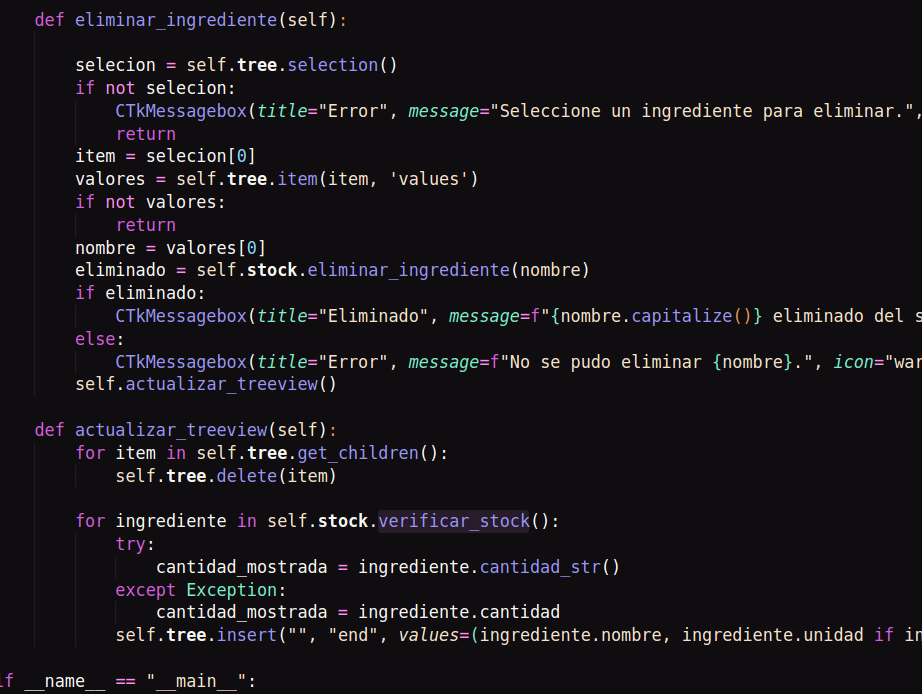
\includegraphics[width=0.8\textwidth]{images/12.png}
    \end{itemize}
\end{itemize}
\newpage
\section{Flujo del Programa Completo}

El programa sigue un flujo lógico dividido en la gestión del inventario y el ciclo de venta, todo orquestado por la clase principal \texttt{AplicacionConPestanas}.

\subsection{Inicio y Gestión de Inventario (Pestañas Stock/Carga)}
\begin{enumerate}
    \item \textbf{Inicialización:} Al iniciar (\texttt{Restaurante.py}), se crea un objeto \texttt{Stock}, el cual automáticamente llama a \texttt{cargar\_desde\_csv} (\texttt{Stock.py}) para recuperar el inventario persistente.
    \item \textbf{Carga Masiva:} En la pestaña ``carga de ingredientes'', el usuario selecciona un archivo CSV. \texttt{Restaurante.py} lee el archivo con \texttt{pandas} y lo muestra en una tabla. Al presionar ``Agregar al Stock'', se itera sobre el \texttt{DataFrame} y se llama a \texttt{stock.agregar\_ingrediente} para cada fila, actualizando la cantidad y persistiendo el cambio con \texttt{stock.actualizar\_csv}.
    \item \textbf{Stock Manual:} En la pestaña ``Stock'', el usuario puede ingresar manualmente un nuevo ingrediente o eliminar uno existente, actualizando la vista \texttt{Treeview} y el archivo CSV.
\end{enumerate}

\subsection{Ciclo de Venta y Descuento de Stock (Pestaña Pedido)}
\begin{enumerate}
    \item \textbf{Generación de Menú (Carta):} El usuario accede a la pestaña ``Pedido'', donde se despliegan las tarjetas de menú generadas a partir de \texttt{Menu\_catalog.py}.
    \item \textbf{Toma de Pedido:} El usuario hace clic en una tarjeta (\texttt{tarjeta\_click}).
    \item \textbf{Verificación y Descuento:}
    \begin{itemize}
        \item Se llama a \texttt{menu.esta\_disponible(stock)}, que verifica si los ingredientes necesarios están en el \texttt{Stock} en la cantidad suficiente.
        \item Si está disponible, el sistema \textbf{descuenta} la cantidad de ingredientes del \texttt{stock.lista\_ingredientes} y llama a \texttt{stock.actualizar\_csv()} para guardar el nuevo estado.
        \item Se añade el menú al objeto \texttt{Pedido} y se actualiza el \texttt{Treeview} del pedido.
    \end{itemize}
    \item \textbf{Total:} Se llama a \texttt{pedido.calcular\_total()} para actualizar el precio mostrado en la GUI.
\end{enumerate}

\subsection{Documentación (Pestañas Carta y Boleta)}
\begin{enumerate}
    \item \textbf{Generar Carta PDF:} En la pestaña ``Carta restorante'', el botón llama a \texttt{create\_menu\_pdf} (\texttt{menu\_pdf.py}), que genera el archivo \texttt{carta.pdf}.
    \item \textbf{Generar Boleta:} Al finalizar el pedido, el botón ``Generar Boleta'' llama a \texttt{BoletaFacade(pedido).generar\_boleta()}. Esta fachada calcula impuestos y detalles, y genera \texttt{boleta.pdf} (\texttt{BoletaFacade.py}).
    \item \textbf{Visualización:} Tanto la Carta como la Boleta se muestran instantáneamente dentro de la aplicación usando el \textit{widget} \texttt{CTkPDFViewer} (\texttt{ctk\_pdf\_viewer.py}), el cual carga el PDF en un hilo separado para una mejor experiencia de usuario.
\end{enumerate}

\end{document}